\documentclass[12pt]{article}
\usepackage[a4paper]{geometry}
\usepackage[myheadings]{fullpage}
\usepackage{fancyhdr}
\usepackage{lastpage}
\usepackage{graphicx, wrapfig, subcaption, setspace, booktabs}
\usepackage[font=small, labelfont=bf]{caption}
\usepackage{fourier}
\usepackage[protrusion=true, expansion=true]{microtype}
\usepackage[english]{babel}
\usepackage[final]{hyperref} 
\usepackage{sectsty}
\usepackage{cite}
\usepackage{url, lipsum}
\usepackage{float}
\usepackage{amsmath}
\usepackage{mathpazo}
\usepackage{mathtools}
\usepackage{multicol}
\usepackage[none]{hyphenat}
\usepackage{siunitx}
\usepackage[RPvoltages]{circuitikz}
\usepackage{gensymb}
\usepackage[framed,numbered]{matlab-prettifier}
\usepackage{chngcntr}
\usepackage[T1]{fontenc}
\usepackage{tabularx}
\usepackage{minted}

\newcommand{\HRule}[1]{\rule{\linewidth}{#1}}
\newcommand*\mean[1]{\overline{#1}}
\onehalfspacing
\setcounter{tocdepth}{5}
\setcounter{secnumdepth}{5}



%-------------------------------------------------------------------------------
% HEADER & FOOTER
%-------------------------------------------------------------------------------
\pagestyle{fancy}
\fancyhf{}
\setlength\headheight{15pt}
\fancyhead[L]{CSCI403 - Project 3 Part 2}
\fancyhead[R]{Ching}
\fancyfoot[R]{Page \thepage\ of \pageref{LastPage}}
%-------------------------------------------------------------------------------
% TITLE PAGE
%-------------------------------------------------------------------------------
\title{\uppercase{CSCI403 - Project 3 Part 2}}
\author{Brandon Ching}



\begin{document}

\section{Introduction}
The timber problem involves a log of wood that is divided into smaller logs of varying sizes. The goal is to find the maximum amount of timber that can be obtained by an individual. In its most basic form, the problem can be solved using a recursive algorithm. However, the recursive algorithm has an exponential time complexity of $O(2^n)$, making it inefficient for large input sizes. To address this issue, a dynamic programming (DP) algorithm can be used to solve the timber problem in $\Theta(n^2)$ time complexity. This report presents the theoretical analysis of the timber problem, the implementation of the recursive and DP algorithms, and an experimental analysis to validate the theoretical results.

\section{Basic Recursive Algorithm}
\label{timber_recursive}
\begin{minted}[linenos]{python}
def timber_recursive(log_sizes):
    # Base Case
    if len(log_sizes) == 1:
        return log_sizes[0]

    # Recursive Case
    return sum(log_sizes) - min(timber_recursive(log_sizes[1:]),
                                timber_recursive(log_sizes[:-1]))
\end{minted}


The timber problem is solvable using a recursive algorithm. With each recursive call, 2 subproblems are created, one with the first log removed and one with the last log removed. Thus the total operations for the recursive algorithm is: $O(2^n)$.

\begin{equation}
    1 + 2 + 2^2 + 2^3 + ... + 2^n = \Theta(2^n)
\end{equation}

\pagebreak
\section{DP Algorithm (Bottom-Up)}
\label{timber_bottom_up}
\begin{minted}[linenos]{python}
def timber_bottom_up(log_sizes):
    '''
    This function solves the timber problem using a bottom-up approach
    :param log_sizes: A list of log sizes
    :return: The maximum value that can be obtained from cutting the logs
    '''
    n = len(log_sizes)
    # Prefix sum of the log sizes
    sums = [0] * n
    for i in range(n):
        sums[i] = log_sizes[i] + (sums[i - 1] if i > 0 else 0)

    # Create a table to store the results and fill in the base case (i == j)
    table = [[0 for _ in range(n)] for _ in range(n)]
    for i in range(n):
        table[i][i] = log_sizes[i]

    # Fill in the table using the bottom-up approach (traverse diagonally)
    for diag in range(1, n):
        for i in range(n - diag):
            j = i + diag
            table[i][j] = sums[j] - (sums[i - 1] if i > 0 else 0) - \
                min(table[i + 1][j], table[i][j - 1])

    return table[0][n - 1]
\end{minted}

The DP bottom-up algorithm solves the timber problem by creating a table to store the results of subproblems. The algorithm fills in the table using a bottom-up approach, starting with the base case (i == j) and then traversing diagonally to fill in the remaining entries. The time complexity of the DP bottom-up algorithm is $\Theta(n^2)$.

At the start of execution, a prefix sum of the log sizes is calculated in $O(n)$ time complexity. The table is then initialized with the base case in $O(n)$ time complexity. The table is filled in using a nested loop that traverses diagonally, with each entry taking $O(1)$ time complexity to calculate and a total of $O(\frac{n^2}{2} - n)$ operations. Thus, the overall time complexity of the DP bottom-up algorithm is $\Theta(n^2)$.

\begin{equation}
    1 + 2 + 3 + ... + n = \Theta(n^2)
\end{equation}

\section{Experimental Analysis}
To validate the theoretical analysis, the DP bottom-up algorithm presented in Section \ref*{timber_bottom_up} was implemented in Python \footnote{Simulation ran on Apple M2 Pro with 16GB unified RAM} and tested with various input sizes, $1 \leq n \leq 2000$. The python random library was used to generate random log sizes for each input size ranging from 1 to 1000. The algorithm was run 100 times for each size and the average time taken to solve the timber problem was recorded for each input size in Table \ref{tab:timber_dp_bottom_up_results} \footnote{Only some of the results are present in the table. The actual simulation tested in intervals of 10}.

\subsection{Experimental Results}
\begin{table}[H]
    \caption{Average time taken to solve the timber problem using the DP bottom-up algorithm}
    \label{tab:timber_dp_bottom_up_results}
    \centering
    \begin{tabular}{|c|c|c|c|}
        \hline
        \textbf{Size} & \textbf{Average Time (ms)} & \textbf{Size} & \textbf{Average Time (ms)} \\
        \hline
        100           & 0.838                      & 1100          & 130.936                    \\ \hline
        200           & 3.253                      & 1200          & 155.425                    \\ \hline
        300           & 7.784                      & 1300          & 185.394                    \\ \hline
        400           & 14.526                     & 1400          & 214.237                    \\ \hline
        500           & 24.288                     & 1500          & 247.649                    \\ \hline
        600           & 35.379                     & 1600          & 283.764                    \\ \hline
        700           & 49.560                     & 1700          & 318.818                    \\ \hline
        800           & 66.870                     & 1800          & 360.112                    \\ \hline
        900           & 85.758                     & 1900          & 402.864                    \\ \hline
        1000          & 106.546                    & 2000          & 442.341                    \\ \hline
    \end{tabular}
\end{table}

\begin{figure}[H]
    \centering
    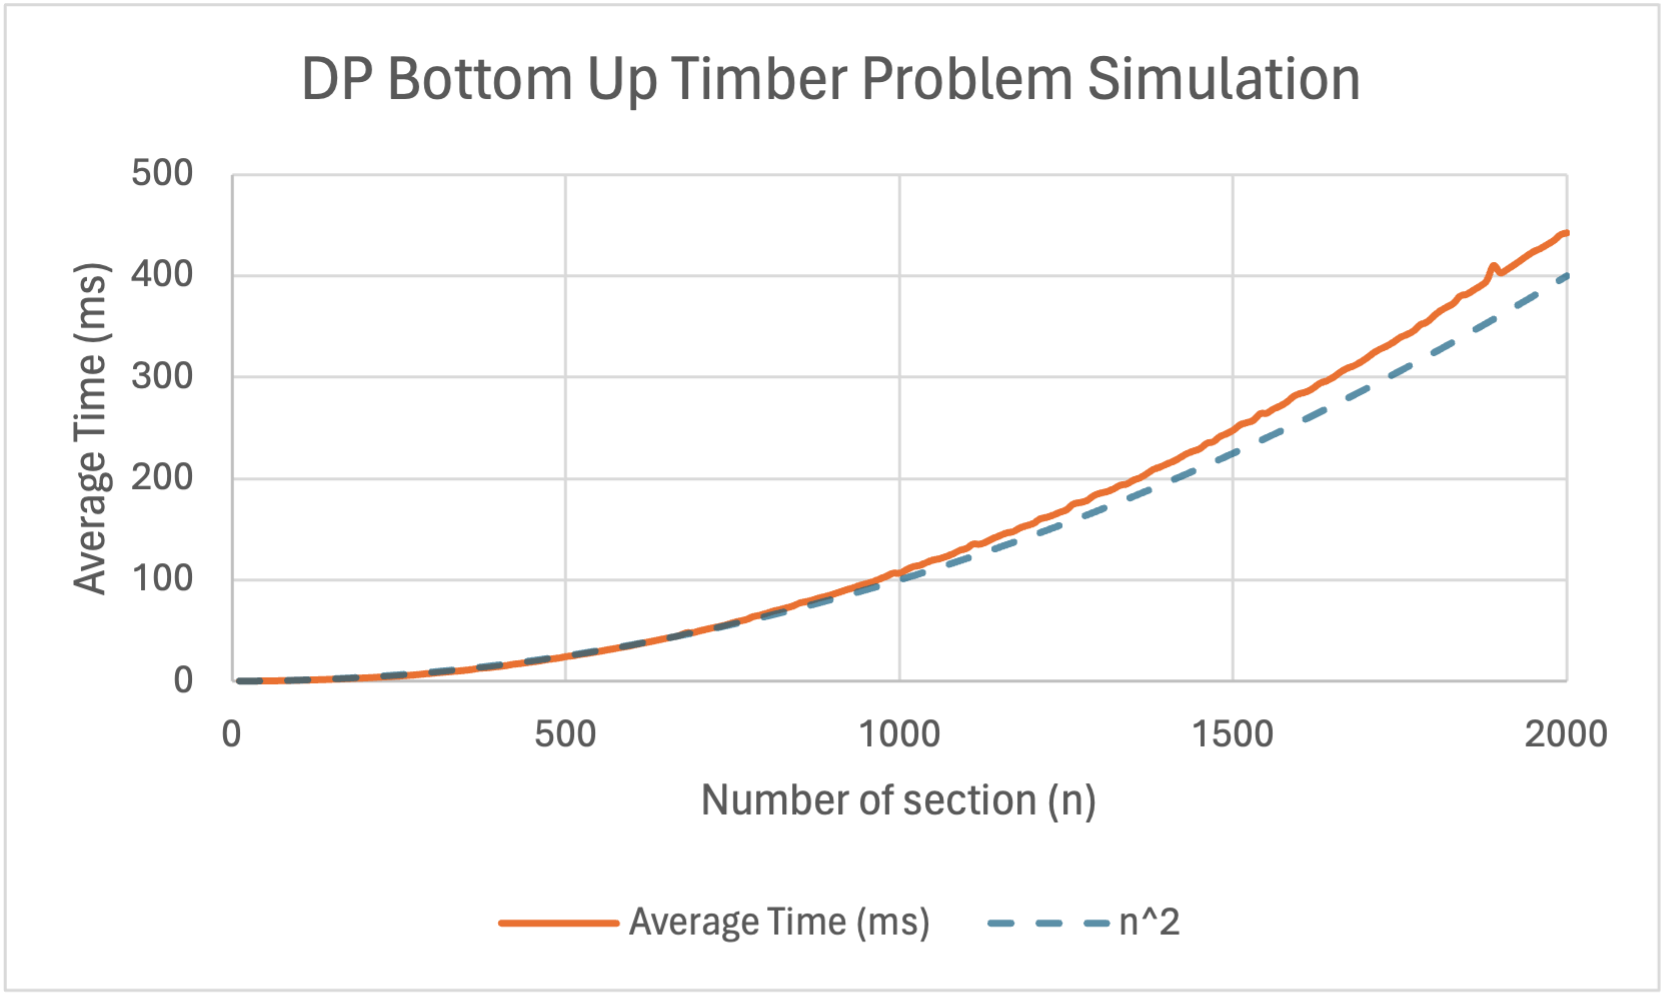
\includegraphics[width=0.8\textwidth]{results_plot.png}
    \caption{Average time taken to solve the timber problem using the  DP bottom-up algorithm}
    \label{fig:timber_dp_bottom_up_results}
\end{figure}

\subsection{Analysis}
The experimental results depicted in Table \ref{tab:timber_dp_bottom_up_results} and Figure \ref{fig:timber_dp_bottom_up_results} showcase a clear trend: the average time taken to solve the timber problem using the DP bottom-up algorithm grows quadratically with the input size.

As shown in Figure \ref{fig:timber_dp_bottom_up_results}, the experimental data closely follows the theoretical analysis of $\Theta(n^2)$\footnote{To provide a more illustrative comparison, a scaled line representing the theoretical complexity ($\Theta(n^2)$) is included in Figure \ref{fig:timber_dp_bottom_up_results}. This scaled line, reduced by a factor of 10,000.}. Despite minor fluctuations in runtime, likely attributable to system variations and other factors, the overall trend exhibits a clear quadratic growth pattern.


\pagebreak
\section{Appendix - Python Code}

\begin{minted}[linenos]{python}
import sys
import random
import time


def timber_recursive(log_sizes):
    '''
    This function solves the timber problem using a recursive approach
    :param log_sizes: A list of log sizes
    :return: The maximum value that can be obtained from cutting the logs
    '''
    # Base Case
    if len(log_sizes) == 1:
        return log_sizes[0]

    # Recursive Case
    return sum(log_sizes) - min(timber_recursive(log_sizes[1:]),
                                timber_recursive(log_sizes[:-1]))


def timber_bottom_up(log_sizes):
    '''
    This function solves the timber problem using a bottom-up approach
    :param log_sizes: A list of log sizes
    :return: The maximum value that can be obtained from cutting the logs
    '''
    n = len(log_sizes)
    # Prefix sum of the log sizes
    sums = [0] * n
    for i in range(n):
        sums[i] = log_sizes[i] + (sums[i - 1] if i > 0 else 0)

    # Create a table to store the results and fill in the base case (i == j)
    table = [[0 for _ in range(n)] for _ in range(n)]
    for i in range(n):
        table[i][i] = log_sizes[i]

    # Fill in the table using the bottom-up approach (traverse diagonally)
    for diag in range(1, n):
        for i in range(n - diag):
            j = i + diag
            table[i][j] = sums[j] - (sums[i - 1] if i > 0 else 0) - \
                min(table[i + 1][j], table[i][j - 1])

    return table[0][n - 1]


def command_line_input():
    '''
    This function reads the input file from the command line and runs 
    the timber_bottom_up function
    :return: None
    '''
    # Get the first argument as the input file
    input_file = sys.argv[1]

    # Read the input file
    with open(input_file, 'r') as f:
        lines = f.readlines()
    f.close()

    # Get the sizes of the logs from the second line and run the algorithm
    log_sizes = list(map(int, lines[1].split()))
    print(timber_bottom_up(log_sizes))


def synthetic_test(max_size=20, test_count=100):
    '''
    This function runs a synthetic test on the timber_recursive function
    The results are written to an output file
    :param range: The range of log sizes to test from 1 to range (default is 20)
    :return: None
    '''
    with open("output_recursive.csv", "w") as f:
        for i in range(1, max_size + 1):
            print("Testing log size: ", i)
            total_time = 0
            for _ in range(test_count):
                # Use a random number generator to generate the log sizes
                log_sizes = [random.randint(1, 1001) for _ in range(i)]
                # Get the start time of the algorithm
                start_time = time.time()
                # Run the algorithm
                timber_recursive(log_sizes)
                # Get the end time of the algorithm
                end_time = time.time()
                # Calculate the time taken in milliseconds
                total_time += (end_time - start_time) * 1000
            # Write the results to the output file
            f.write(f"{i}, {total_time / test_count}\n")
    f.close()


def synthetic_test_bottom_up(max_size=2000, test_count=100):
    '''
    This function runs a synthetic test on the timber_bottom_up function
    The results are written to an output file
    :param range: The range of log sizes to test (default is 2000)
    :return: None
    '''
    with open("output_bottom_up.csv", "w") as f:
        for i in range(1, max_size + 1):
            print("Testing log size: ", i)
            total_time = 0
            for _ in range(test_count):
                # Use a random number generator to generate the log sizes
                log_sizes = [random.randint(1, 1001) for _ in range(i)]
                # Get the start time of the algorithm
                start_time = time.time()
                # Run the algorithm
                timber_bottom_up(log_sizes)
                # Get the end time of the algorithm
                end_time = time.time()
                # Calculate the time taken in milliseconds
                total_time += (end_time - start_time) * 1000
            # Write the results to the output file
            f.write(f"{i}, {total_time / test_count}\n")
    f.close()


def validate_methods():
    '''
    This function validates the timber_recursive and timber_bottom_up 
    functions by comparing the results for random log sizes
    :return: None
    '''
    # Test random log lengths and random log sizes for 1000 iterations
    for _ in range(1000):
        if _ % 100 == 0:
            print(f"Testing iteration: {_}")
        log_sizes = [random.randint(1, 1001)
                     for _ in range(random.randint(1, 21))]
        # print if the results are not the same
        if timber_recursive(log_sizes) != timber_bottom_up(log_sizes):
            print("Results are not the same")
            print(log_sizes)
            print(timber_recursive(log_sizes))
            print(timber_bottom_up(log_sizes))
            return


if __name__ == "__main__":
    # Uncomment the line below to run the command line input
    command_line_input()  # This one is used for grading
    # synthetic_test()
    # synthetic_test_bottom_up()
    # validate_methods()

\end{minted}



\end{document}